\documentclass[a4paper,10pt,landscape,twocolumn]{scrartcl}

%% Settings
\newcommand\problemset{2}
\newif\ifcomments
\commentsfalse % hide comments
%\commentstrue % show comments

%% Packages
\usepackage[english]{exercises}
\usepackage{wasysym}
\usepackage{graphicx}
\usepackage{hyperref}
\hypersetup{colorlinks=true, urlcolor = blue, linkcolor = blue}

%% Macros
\usepackage{xspace}

\newcommand{\eps}{\varepsilon}
\newcommand{\ket}[1]{|#1\rangle}
\newcommand{\bra}[1]{\langle#1|}
\newcommand{\inp}[2]{\langle{#1}|{#2}\rangle}
\newcommand{\norm}[1]{\parallel\!#1\!\parallel}
\newcommand{\points}[1]{\marginpar{\textbb{#1 p.}}}
\newtheorem{theorem}{Theorem}
\newtheorem{definition}{Definition}
\newtheorem{proposition}{Proposition}
%\newenvironment{proof}{\noindent {\bf Proof }}{{\hfill $\Box$}\\}

\newcommand{\gen}{\ensuremath{\mathsf{Gen}}\xspace}
\newcommand{\enc}{\ensuremath{\mathsf{Enc}}\xspace}
\newcommand{\dec}{\ensuremath{\mathsf{Dec}}\xspace}
\newcommand{\mac}{\ensuremath{\mathsf{Mac}}\xspace}
\newcommand{\vrfy}{\ensuremath{\mathsf{Vrfy}}\xspace}
\newcommand{\negl}{\ensuremath{\mathsf{negl}}\xspace}
\newcommand{\PrivK}{\ensuremath{\mathsf{PrivK}}\xspace}
\newcommand{\eav}{\ensuremath{\mathsf{eav}}\xspace}

\newcommand{\Z}{\ensuremath{\mathbb{Z}}}
\newcommand{\R}{\ensuremath{\mathbb{R}}}
\newcommand{\N}{\ensuremath{\mathbb{N}}}


\newcommand\floor[1]{\lfloor#1\rfloor}
\newcommand\ceil[1]{\lceil#1\rceil}

% \newcommand{\comment}[1]{{\sf [#1]}\marginpar[\hfill !!!]{!!!}}
\newcommand{\chris}[1]{\comment{\color{blue}Chris: #1}}
\newcommand{\jan}[1]{\comment{\color{magenta}Jan: #1}}


\begin{document}

\problems

%{\sffamily\noindent
%We will work on the following exercises together during the work session on Tuesday, 12 Sep 2017.
%
% }




\begin{figure}[h]
\center
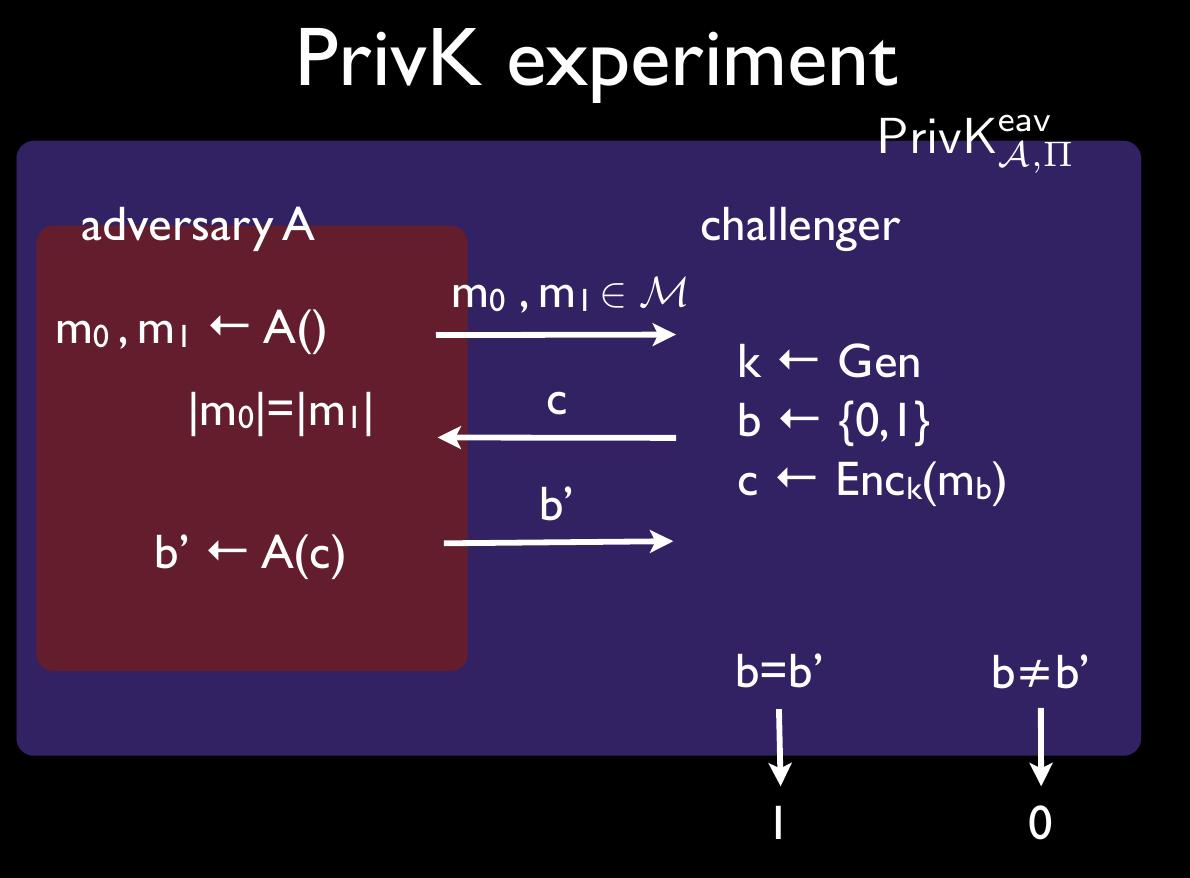
\includegraphics[width=8cm]{PrivKexperiment.jpg}
\caption{The $\PrivK^{\eav}_{\mathcal{A},\Pi}$ experiment \label{fig:privk-eav}}
\end{figure}

\begin{exercise}[The $\PrivK^{\eav}_{\mathcal{A},\Pi}$ experiment (see Figure~\ref{fig:privk-eav})]
For each of the following scenarios, give the maximal value of $\Pr[\PrivK^{\eav}_{\mathcal{A},\Pi}=1]$ and explain how it can be achieved.

\begin{subex}
Let $\Pi$ be the shift cipher, and let us consider an adversary $\mathcal{A}$ that submits $m_0 = \mathtt{a}$ and $m_1 = \mathtt{a}$.
\end{subex}

\begin{subex}
Let $\Pi$ be the shift cipher, and let us consider an adversary $\mathcal{A}$ that submits $m_0 = \mathtt{a}$ and $m_1 = \mathtt{b}$.
\end{subex}

\begin{subex}
Let $\Pi$ be the shift cipher, and let us consider an adversary $\mathcal{A}$ that submits $m_0 = \mathtt{aa}$ and $m_1 = \mathtt{bb}$.
\end{subex}

\begin{subex}
Let $\Pi$ be the shift cipher, and let us consider an adversary $\mathcal{A}$ that submits $m_0 = \mathtt{aa}$ and $m_1 = \mathtt{ab}$.
\end{subex}

\begin{subex}
Let $\Pi$ be the one-time-pad encryption of three-letter messages, and let us consider an adversary $\mathcal{A}$ that submits $m_0 = \mathtt{aaa}$ and $m_1 = \mathtt{abc}$.
\end{subex}

\begin{subex}
Let $\Pi$ be the monoalphabetic substitution cipher. Give an adversary $\mathcal{A}$ that manages to win the $\PrivK^{\eav}_{\mathcal{A},\Pi}$ experiment all the time, i.e.\ such that $\Pr[\PrivK^{\eav}_{\mathcal{A},\Pi}=1] = 1$.
\end{subex}
\end{exercise}


\begin{exercise}[Negligible functions]
Recall Definition 3.4: A function $f: \Z^+ \rightarrow \R^+$ is called \emph{negligible} if for
every positive polynomial $p(n)$ there exists $N \in \Z^+$ such that for all integers $n> N$, it holds that $f(n) < \frac{1}{p(n)}$.

\begin{subex}
Example~3.5 states that $f(n) = 2^{-\sqrt{n}}$ is negligible. For the polynomial $p(n)=16 n^4$, give a possible $N$ as in the definition above, i.e.\ such that for all integers $n > N$, it holds that $f(n) < \frac{1}{p(n)}$.
\end{subex}

\begin{subex}
Example~3.5 states that $f(n) = n^{-\log{n}}$ is negligible. For the polynomial $p(n)=16 n^4$, give a possible $N$ as in the definition above, i.e.\ such that for all integers $n > N$, it holds that $f(n) < \frac{1}{p(n)}$.
\end{subex}

\begin{subex**}
Let $\negl_1$ and $\negl_2$ be negligible functions. Prove that the function $\negl_3$ defined by $\negl_3(n) = \negl_1(n)+\negl_2(n)$ is negligible.
\end{subex**}

\begin{subex**}
For any positive polynomial $p$, the function $\negl_4$ defined
  by $\negl_4(n) = p(n) \cdot \negl_1(n)$ is negligible.
\end{subex**}

\end{exercise}


\begin{exercise}[not PRGs]
For all of the following constructions, explain why they are not PRGs.
Can you give an explicit description of an efficient distinguisher in
each case?

\begin{subex}
Let $G(s)$ output $s$.
\end{subex}

\begin{subex}
Let $G(s)$ output $s \| s$
\end{subex}

\begin{subex}
Let $G(s)$ output $s \| \bigoplus_{i=1}^n s_i$.
\end{subex}

\end{exercise}

\begin{exercise}[Basic properties of PRGs]
Recall that the \href{https://en.wikipedia.org/wiki/Image_(mathematics)}{\emph{image} of a function} $f:A \rightarrow B$ is the subset $f(A)$ of $B$. Formally,
\[ \mathsf{im}(f) := f(A) = \{b \in B \mid \exists a \in A \mbox{ such that } b=f(a) \} \, .
\]

Let $G:\{0,1\}^n \rightarrow \{0,1\}^{2n}$ be a PRG.

\begin{subex}
Let us assume that $G$ is \href{https://en.wikipedia.org/wiki/Injective_function}{injective}. How many different $2n$-bit strings $y$ are there in the image of $G$?
\end{subex}

\begin{subex}
What is the fraction of images of $G$ among all $2n$-bit strings?
\end{subex}

\begin{subex}
For a given $y \in \{0,1\}^{2n}$, what is $\Pr_{s \leftarrow
  \{0,1\}^n}[G(s) = y]$? Express this probability in terms of $|\{s \in \{0,1\}^n \mid G(s)=y\} |$ and $n$.
\end{subex}

\end{exercise}

\begin{figure}[h]
\center
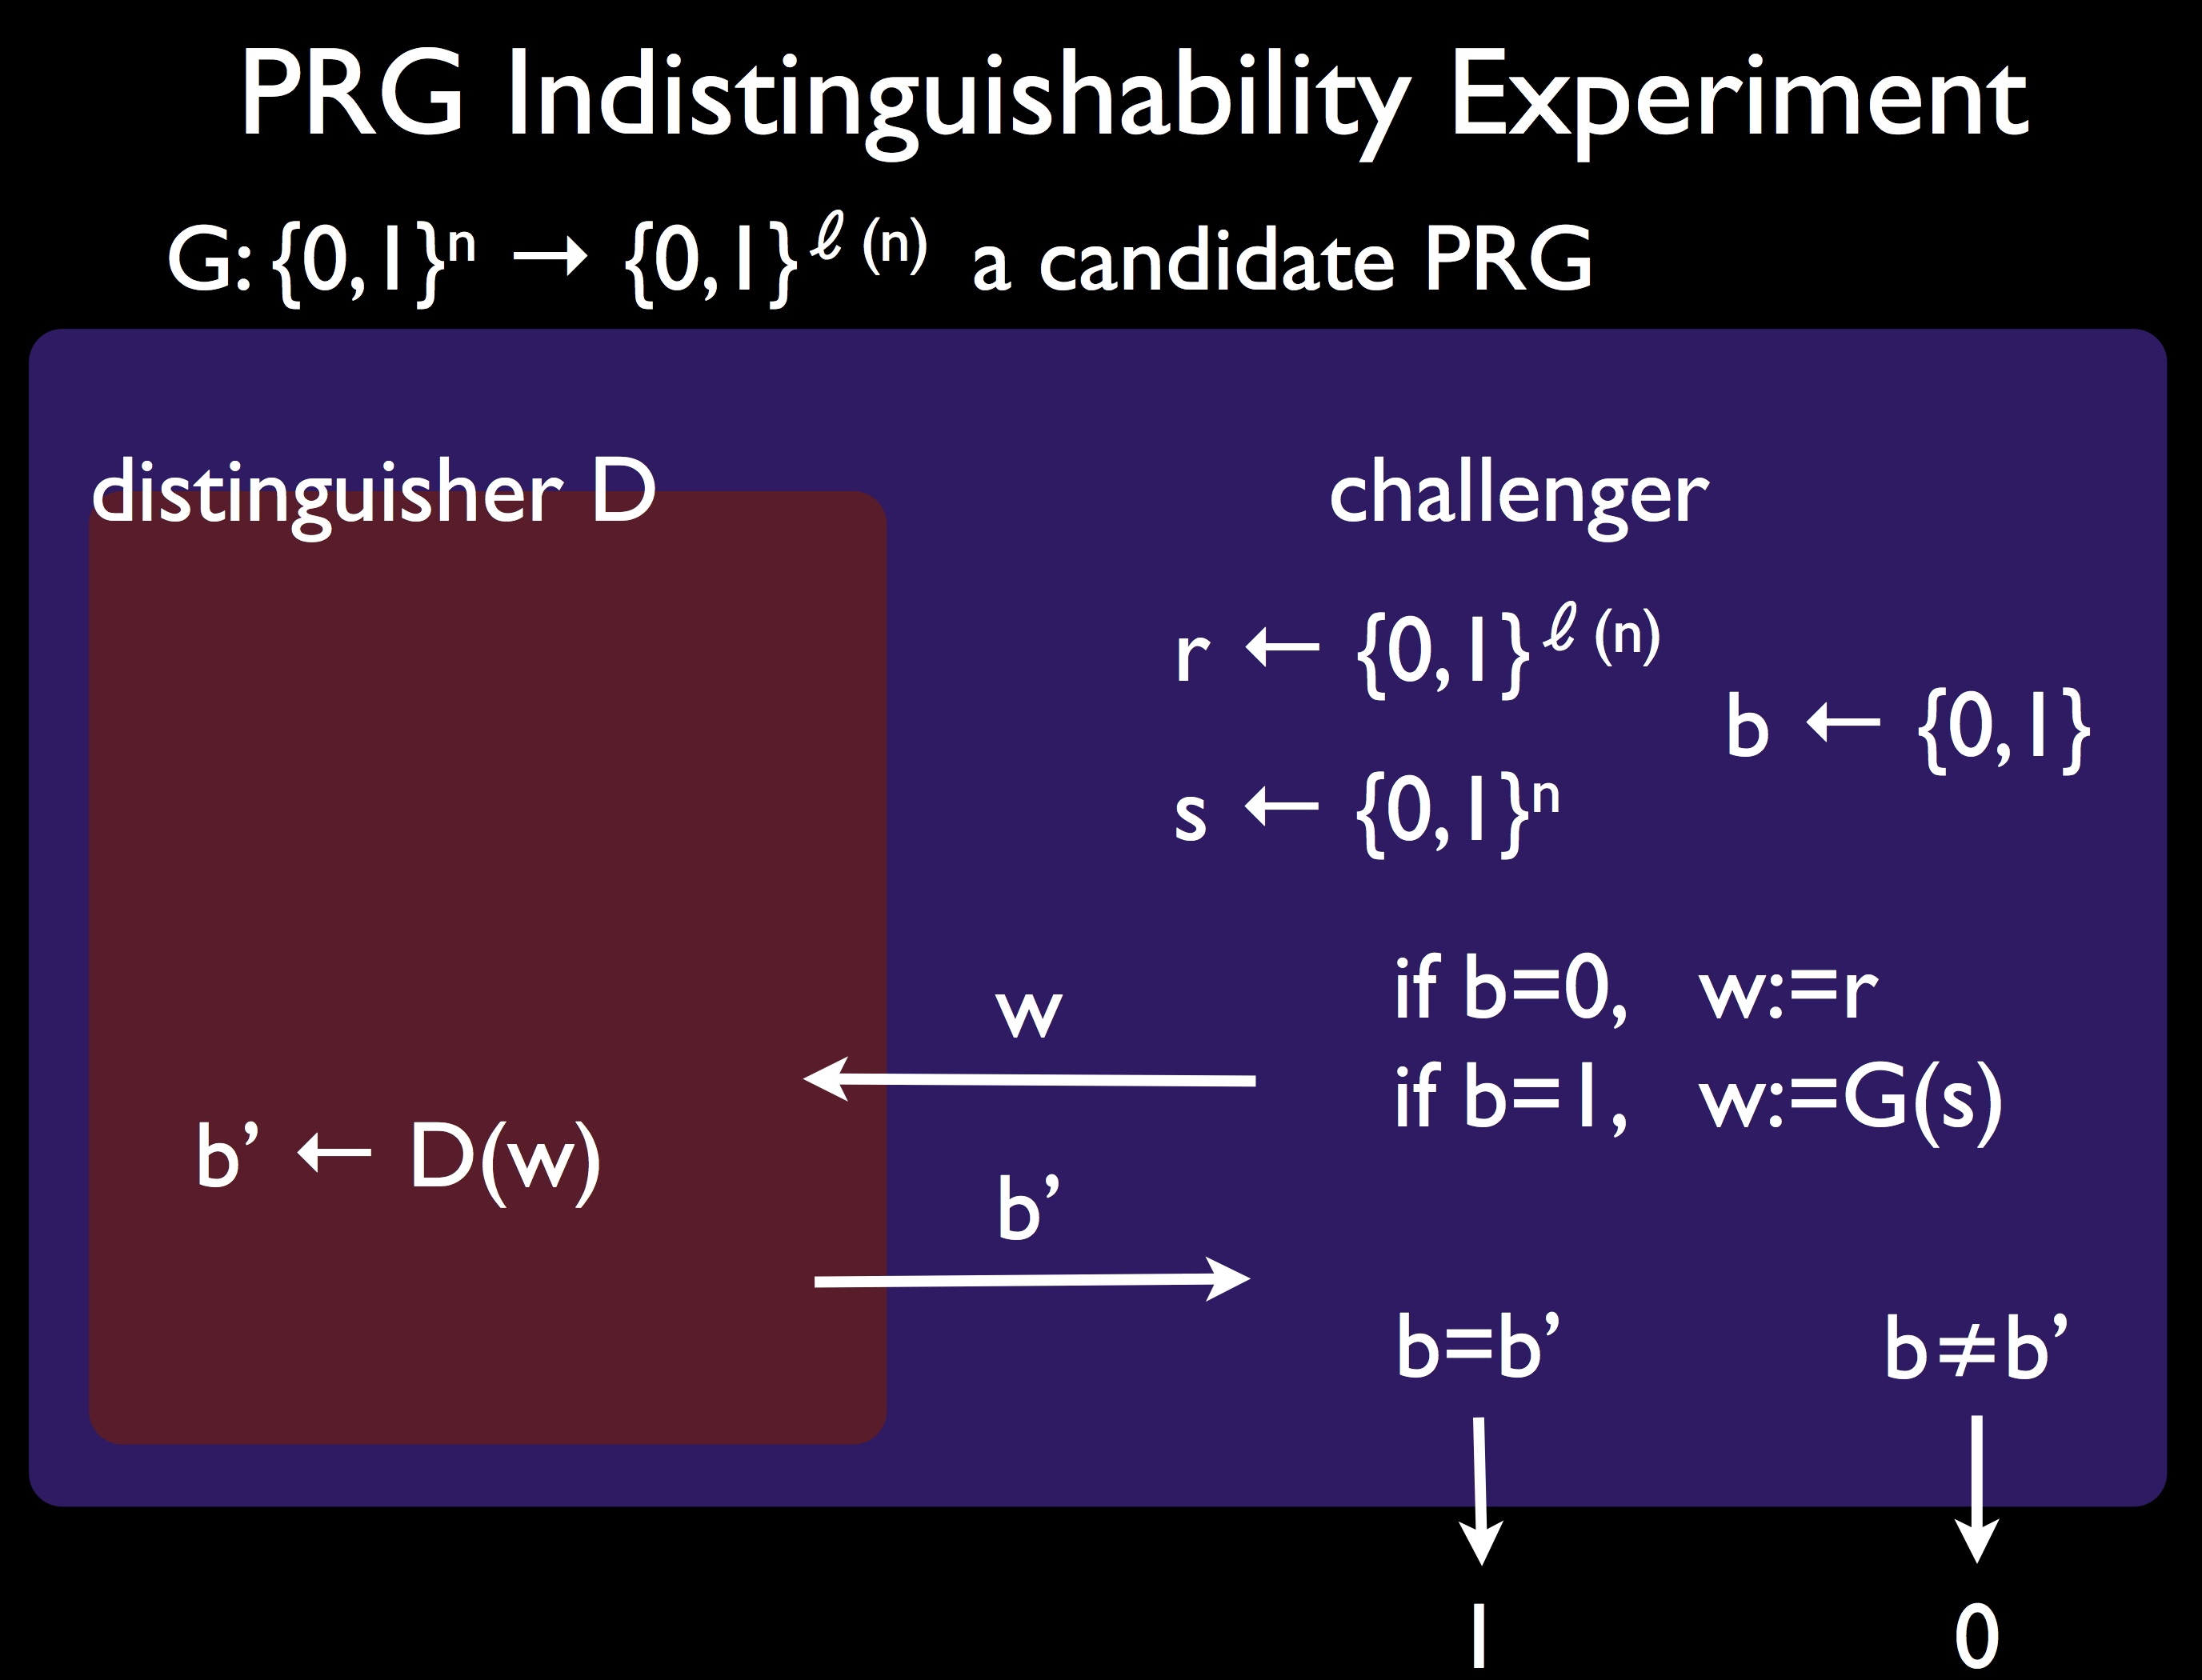
\includegraphics[width=8cm]{PRGExperiment.jpg}
\caption{The $\mathsf{PRG}_{\mathcal{D},G}$ experiment \label{fig:prg-exp}}
\end{figure}

\begin{exercise}[Exercise~3.5 from  $\text{[KL]}$ ]
  Let $|G(s)| = \ell(|s|)$ for some $\ell$. Consider the following experiment:

  \textbf{The PRG indistinguishability experiment} $\mathsf{PRG}_{\mathcal{A},G}(n)$, see also Figure~\ref{fig:prg-exp}:
  \textit{
  \begin{enumerate}[label=(\alph*)]
\item  A uniform bit $b \in \{0,1\}$ is chosen. If $b = 0$ then choose a uniform $r \leftarrow \{0, 1\}^{\ell(n)}$ and set $w:=r$; if $b = 1$ then choose a uniform $s \leftarrow \{0,1\}^n$ and set $w := G(s)$.
\item The adversary $\mathcal{A}$ is given $w$, and outputs a bit $b'$.
\item The output of the experiment is defined to be 1 if $b' = b$,
  and 0 otherwise.
  \end{enumerate}
  }
Provide a definition of a pseudorandom generator based on this experiment, and prove that your definition is equivalent to Definition 3.14. (That is, show that $G$ satisfies your definition if and only if it satisfies Definition 3.14.)

\end{exercise}


\begin{exercise}[Exercise~3.2 from $\text{[KL]}$ ]
Prove that Definition~3.8 cannot be
  satisfied if $\Pi$ can encrypt arbitrary-length messages and the
  adversary is not restricted to output equal-length messages in
  experiment $\PrivK^{\eav}_{\mathcal{A},\Pi}$. \textbf{ Hint:} Let $q(n)$
  be a polynomial upper-bound on the length of the cipher-text when
  $\Pi$ is used to encrypt a single bit. Then consider an adversary
  who outputs $m_0 \in \{0, 1\}$ and a uniform $m_1 \in \{0, 1\}^{q(n)+1}$.
\end{exercise}

% \begin{exercise}[Exercise~3.3 from  $\text{[KL]}$ ]
% Say $\Pi=\left( \gen,\enc,\dec \right)$ is such that for $k\in \{0,1\}^n$, algorithm $\enc_k$ is only defined for messages of length at most $\ell(n)$ (for some polynomial $\ell$). Construct a scheme satisfying Definition~3.8 even when the adversary is \emph{not} restricted to outputting equal-length messages in $\PrivK^{\eav}_{\mathcal{A},\Pi}$.
% \end{exercise}

\begin{bonusexercise}[Exercise~3.4 from  $\text{[KL]}$ ]
Prove the equivalence of Definition 3.8 and Definition 3.9 from the book [KL].
\end{bonusexercise}

%\pagebreak
% \begin{bonusexercise}[Brute-forcing a PRG]
% Let $G:\{0,1\}^n \rightarrow \{0,1\}^{2n}$ be a PRG. Describe a \emph{computationally unbounded} adversary $\mathcal{A}$ that distinguishes the output of $G$ from a uniform $2n$-bit string with probability exponentially close 1. How does it work? Compute its exact distinguishing advantage. What is $\Pr[\mathsf{PRG}_{\mathcal{A},G}(n)=1]$ for this adversary?
% \end{bonusexercise}

\begin{bonusexercise}[Exercise~3.7 from $\text{[KL]}$ ]
Prove the converse of Theorem 3.18. Namely, show that if $G$ is not a pseudorandom generator then Construction 3.17 does not have indistinguishable encryptions in the presence of an eavesdropper.
\end{bonusexercise}


\end{document}
